\documentclass[a4paper]{article}

\usepackage[margin=1in]{geometry}
\usepackage{graphicx}
\usepackage{booktabs}
\usepackage{tikz}
\usepackage{pgfplots}
\usepackage{paralist}
\pgfplotsset{compat=1.16}

\begin{document}

\section*{Chosen Discovery Algorithms}
For this factor analysis, you chose the following miners to discover process models:
\begin{compactitem}
\item Alpha miner
\end{compactitem}

This means, for each input event log, the program discovered models using each of the aforementioned discovery algorithms.
For the resulting Petri nets, it calculated the complexity score of each selected measure, which formed the population.

You chose to analyze the following complexity measures:
\begin{compactitem}
\item Size
\item Connector Mismatch
\item Connector Heterogeneity
\item Token split
\item Control flow complexity
\item Separability
\item Average connector degree
\item Maximum connector degree
\item Sequentiality
\item Coefficient of network connectivity
\item Density
\item Number of duplicate tasks
\item Number of empty sequence flows
\end{compactitem}

\section*{Validity of the Factor Analysis}
Your sample size in this analysis was $288$.
It is recommended to have a sample size of at least $5 \cdot 13 = 65$.

Bartlett's test of sphericity returned a $\chi^2$ value of $5582.073608641951$ and a $p$-value of $0.0$.
This means, the variables are probably correlated and we can perform a factor analysis.

The measure of sampling adequacy (MSA) returned the following results:
\begin{compactitem}
\item Size: $0.8346$
\item Connector Mismatch: $0.9447$
\item Connector Heterogeneity: $0.6137$
\item Token split: $0.8972$
\item Control flow complexity: $0.8792$
\item Separability: $0.7386$
\item Average connector degree: $0.6216$
\item Maximum connector degree: $0.8662$
\item Sequentiality: $0.7672$
\item Coefficient of network connectivity: $0.9163$
\item Density: $0.6276$
\item Number of empty sequence flows: $0.8824$
\item overall MSA: $0.8338781943194749$
\end{compactitem}

\section*{Chosen Number of Factors}
The Scree test resulted in the following Eigenvalue plot:
\begin{center}
\begin{tikzpicture}
\begin{axis}[xtick=data,width=15cm,height=8cm]
\addplot [draw=cyan!50!blue, mark=*] coordinates { (1,0.5673) (2,0.1923) (3,0.1) (4,0.0563) (5,0.0441) (6,0.0132) (7,0.0108) (8,0.0078) (9,0.0039) (10,0.0023) (11,0.0013) (12,0.0008)};
\end{axis}
\end{tikzpicture}
\end{center}
You choose to set the number of expected factors to $4$.

\section*{Descriptive Statistics}
\begin{center}
\begin{tabular}{lrrrrr}
\toprule
 & Mean & Median & Std & Min & Max \\
\midrule
Size & 63.444444 & 65.000000 & 30.159224 & 17.000000 & 157.000000 \\
Connector Mismatch & 12.486111 & 8.000000 & 12.730378 & 0.000000 & 66.000000 \\
Connector Heterogeneity & 0.917159 & 0.939010 & 0.105722 & 0.000000 & 1.000000 \\
Token split & 38.607639 & 33.000000 & 38.004340 & 0.000000 & 193.000000 \\
Control flow complexity & 52.343750 & 49.000000 & 40.718588 & 3.000000 & 228.000000 \\
Separability & 0.928865 & 0.969923 & 0.122749 & 0.235294 & 1.000000 \\
Average connector degree & 4.557755 & 4.548589 & 1.032176 & 2.833333 & 11.500000 \\
Maximum connector degree & 10.961806 & 11.000000 & 4.758480 & 3.000000 & 26.000000 \\
Sequentiality & 0.946049 & 0.994126 & 0.106448 & 0.375000 & 1.000000 \\
Coefficient of network connectivity & 1.707149 & 1.707692 & 0.454102 & 0.941176 & 3.012739 \\
Density & 0.070863 & 0.056194 & 0.043678 & 0.039332 & 0.383333 \\
Number of duplicate tasks & 0.000000 & 0.000000 & 0.000000 & 0.000000 & 0.000000 \\
Number of empty sequence flows & 28.555556 & 27.000000 & 25.006279 & 0.000000 & 113.000000 \\
\bottomrule
\end{tabular}
\end{center}

\section*{Results of the Factor Analysis}
\begin{center}
\begin{tabular}{ccccc} \toprule 
 & Factor 1 & Factor 2 & Factor 3 & Factor 4 \\ \midrule 
Size & $0.9419$ & \textcolor{lightgray}{$-0.1856$} & \textcolor{lightgray}{$0.2135$} & \textcolor{lightgray}{$-0.0609$} \\ 
Connector Mismatch & $0.5648$ & \textcolor{lightgray}{$-0.021$} & \textcolor{lightgray}{$0.1702$} & \textcolor{lightgray}{$0.1525$} \\ 
Connector Heterogeneity & \textcolor{lightgray}{$-0.0756$} & $-0.4894$ & \textcolor{lightgray}{$0.0306$} & $0.6223$ \\ 
Token split & $0.9709$ & \textcolor{lightgray}{$0.0231$} & \textcolor{lightgray}{$0.1405$} & \textcolor{lightgray}{$-0.1295$} \\ 
Control flow complexity & $0.9682$ & \textcolor{lightgray}{$0.0149$} & \textcolor{lightgray}{$0.1949$} & \textcolor{lightgray}{$-0.032$} \\ 
Separability & \textcolor{lightgray}{$0.2627$} & \textcolor{lightgray}{$-0.0503$} & $0.9279$ & \textcolor{lightgray}{$-0.0967$} \\ 
Average connector degree & \textcolor{lightgray}{$0.278$} & $0.9024$ & \textcolor{lightgray}{$0.1998$} & \textcolor{lightgray}{$-0.1098$} \\ 
Maximum connector degree & $0.7951$ & $0.4146$ & \textcolor{lightgray}{$0.2369$} & \textcolor{lightgray}{$0.0408$} \\ 
Sequentiality & $0.3538$ & \textcolor{lightgray}{$0.2991$} & $0.7586$ & \textcolor{lightgray}{$0.2011$} \\ 
Coefficient of network connectivity & $0.921$ & \textcolor{lightgray}{$0.1027$} & \textcolor{lightgray}{$0.3048$} & \textcolor{lightgray}{$0.0255$} \\ 
Density & $-0.4282$ & $0.8121$ & \textcolor{lightgray}{$-0.0496$} & \textcolor{lightgray}{$-0.1656$} \\ 
Number of empty sequence flows & $0.9718$ & \textcolor{lightgray}{$-0.0117$} & \textcolor{lightgray}{$0.1912$} & \textcolor{lightgray}{$-0.0869$} \\ 
\bottomrule
\end{tabular}
\end{center}

\section*{Communalities}
\begin{center}
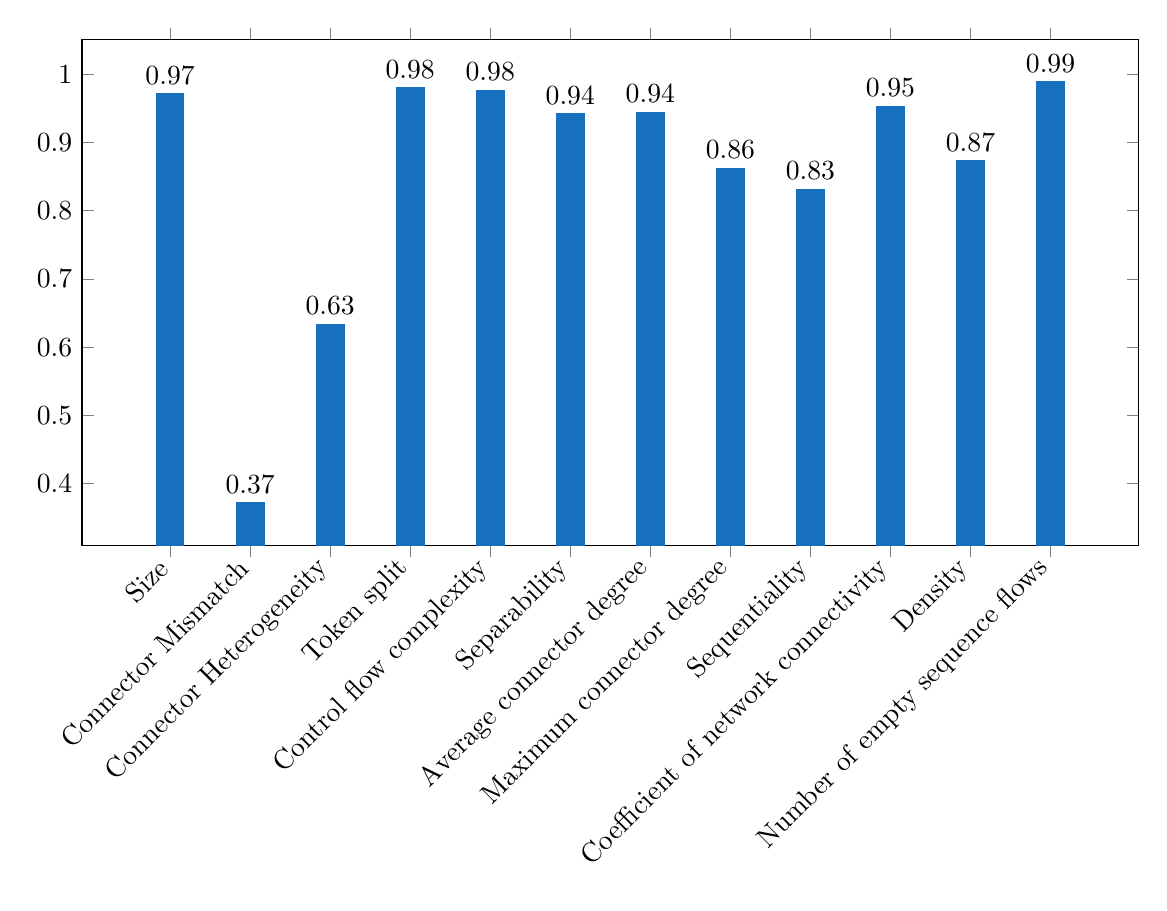
\begin{tikzpicture}
\begin{axis}[ybar,symbolic x coords={Size,Connector Mismatch,Connector Heterogeneity,Token split,Control flow complexity,Separability,Average connector degree,Maximum connector degree,Sequentiality,Coefficient of network connectivity,Density,Number of empty sequence flows},xtick=data,xticklabel style={rotate=45, anchor=east},nodes near coords={\pgfmathprintnumber{\pgfplotspointmeta}},width=15cm,height=8cm]
\addplot [draw=cyan!50!blue, fill=cyan!50!blue] plot coordinates { (Size,0.971) (Connector Mismatch,0.3716) (Connector Heterogeneity,0.6333) (Token split,0.9798) (Control flow complexity,0.9766) (Separability,0.9418) (Average connector degree,0.9436) (Maximum connector degree,0.8618) (Sequentiality,0.8306) (Coefficient of network connectivity,0.9524) (Density,0.8727) (Number of empty sequence flows,0.9886)};
\end{axis}
\end{tikzpicture}
\end{center}

\end{document}
